\begin{name}
	{\tenchude}
	{ĐỀ ÔN TẬP CHƯƠNG I}
	{LỚP TOÁN THẦY PHÁT}
	{\thoigian}
\end{name}

\TN
\Opensolutionfile{ans}[ans/ansc101]
\Opensolutionfile{ans}[ans/ansDe1-TN1]
\begin{ex}%[2D1H5-3]
	Cho hàm số $y=f(x)$ có đồ thị như hình. Tìm số nghiệm của phương trình $2f(x)+3=0$.
	\begin{center}
		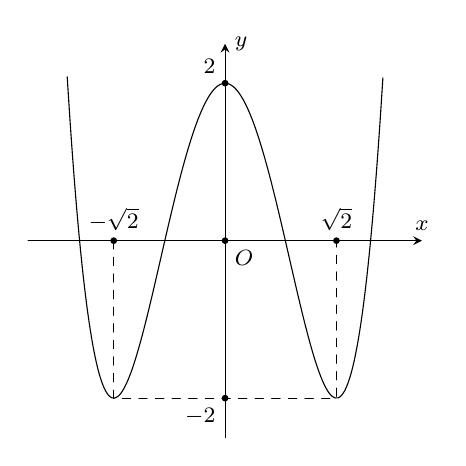
\begin{tikzpicture}[line join=round, line cap = round, >=stealth, scale=1,font=\footnotesize,transform shape]
			\pgfmathsetmacro\a{sqrt(2)}
			\draw[->] (-2.5,0) -- (2.5,0)node[above]{$x$};
			\draw[->] (0,-2.5) -- (0,2.5)node[right]{$y$};
			%\draw[-] (-2.1,-1.5) -- (2.2,-1.5) node[right]{$y=-\frac{3}{2}$};
			\draw[fill=black]
			(0,0) circle(1pt) node[below right]{$O$}
			(0,2) circle(1pt) node[above left]{$2$}
			(0,-2) circle(1pt) node[below left]{$-2$}
			(-\a,0) circle(1pt) node[above]{$-\sqrt{2}$}
			(\a,0) circle(1pt) node[above]{$\sqrt{2}$}
			;
			\draw[dashed]
			(-\a,0)--(-\a,-2)--(\a,-2)--(\a,0)
			;
			\draw[smooth,samples=100,domain=-2.005:2.005] plot(\x,{(\x)^4-4*(\x)^2+2});
		\end{tikzpicture}
	\end{center}
	\choice
	{\True $4$}
	{$2$}
	{$0$}
	{$3$}
	\loigiai{
		Ta có $2f(x)+3=0 \Leftrightarrow f(x)=-\dfrac{3}{2}.\quad (*)$
		\begin{center}
			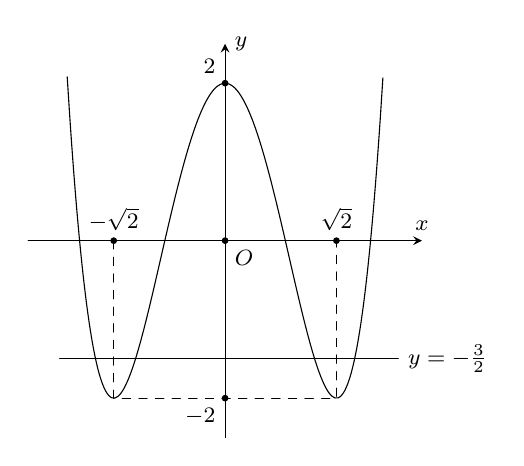
\begin{tikzpicture}[line join=round, line cap = round, >=stealth, scale=1,font=\footnotesize,transform shape]
				\pgfmathsetmacro\a{sqrt(2)}
				\draw[->] (-2.5,0) -- (2.5,0)node[above]{$x$};
				\draw[->] (0,-2.5) -- (0,2.5)node[right]{$y$};
				\draw[-] (-2.1,-1.5) -- (2.2,-1.5) node[right]{$y=-\frac{3}{2}$};
				\draw[fill=black]
				(0,0) circle(1pt) node[below right]{$O$}
				(0,2) circle(1pt) node[above left]{$2$}
				(0,-2) circle(1pt) node[below left]{$-2$}
				(-\a,0) circle(1pt) node[above]{$-\sqrt{2}$}
				(\a,0) circle(1pt) node[above]{$\sqrt{2}$}
				;
				\draw[dashed]
				(-\a,0)--(-\a,-2)--(\a,-2)--(\a,0)
				;
				\draw[smooth,samples=100,domain=-2.005:2.005] plot(\x,{(\x)^4-4*(\x)^2+2});
			\end{tikzpicture}
		\end{center}
		Số nghiệm của phương trình $(*)$ là số giao điểm của đồ thị hàm số $f(x)$ và đường thẳng nằm ngang $y=-\dfrac{3}{2}$. Quan sát hình vẽ, nhận thấy số giao điểm là $4$. Suy ra số nghiệm của phương trình là $4$.
	}
\end{ex}

\begin{ex}%[2D1N5-3]
	\immini
	{
		Cho hàm số có đồ thị là đường cong trong hình bên. Tọa độ giao điểm của đồ thị hàm số đã cho và trục tung là
		\choice
		{$(0;-2)$}
		{$(-1;0)$}
		{\True $(0;-1)$}
		{$(-2;0)$}
	}
	{
		\begin{tikzpicture}[>=stealth,x=1cm,y=1cm,scale=1,font=\footnotesize,line cap=round,line join=round]
			\draw[->] (-2.5,0)--(0,0)%
			node[below right]{$O$}--(2.5,0) node[below]{$x$};
			\draw[->] (0,-3) --(0,2) node[right]{$y$};
			\foreach \x in {-2,2}{
					\draw[fill=black] (\x,0) node[above]{$\x$} circle (1pt);%Ox
				}
			\foreach \y in {-2}{
					\draw[fill=black] (0,\y) node[below left]{$\y$} circle (1pt);%Oy
				}
			\draw[fill=black] (0,-1) node[above left]{$-1$} circle (1pt) (0,1) node[left] {$1$} circle (1pt);
			\draw [domain=-1.7:1.7, samples=100]%
			plot (\x, {(\x)^4-2*(\x)^2-1});
			\draw [dashed] (1,0) node[above]{$1$}%
			--(1,-2)--(-1,-2)--(-1,0)
			node[above]{$-1$};
			\draw[fill=black] (0,0) circle(1pt);
		\end{tikzpicture}
	}
	\loigiai{
		Từ đồ thị ta thấy đồ thị hàm số cắt trục tung tại điểm có tọa độ $(0;-1)$.
	}
\end{ex}

\begin{ex}%[2D1V5-4]
	Cho hàm số $y=x^3-3mx^2+\left(3m-1\right)x+6m$ có đồ thị là $(C)$. Tìm tất cả các giá trị thực của tham số $m$ để $(C)$ cắt trục hoành tại ba điểm phân biệt có hoành độ $x_1, x_2, x_3$ thỏa mãn điều kiện $x_1^2+x_2^2+x_3^2+x_1x_2x_3=20$.
	\choice
	{$m=\dfrac{3\pm \sqrt{33}}{3}$}
	{$m=\dfrac{2\pm \sqrt{3}}{3}$}
	{$m=\dfrac{5\pm \sqrt{5}}{3}$}
	{\True $m=\dfrac{2\pm \sqrt{22}}{3}$}
	\loigiai{
		Phương trình hoành độ giao điểm của $(C)$ và trục hoành là
		\begin{eqnarray*}
			& & x^3-3mx^2+\left(3m-1\right)x+6m=0\\
			&\Leftrightarrow & \left(x+1\right)\left(x^2-\left(3m+1\right)x+6m\right)=0\\
			&\Leftrightarrow & \hoac{& x=-1=x_3 \\
				& g(x)=x^2-\left(3m+1\right)x+6m=0.\quad (*)
			}
		\end{eqnarray*}
		Điều kiện để $(C)$ cắt trục hoành tại ba điểm phân biệt có hoành độ $x_1, x_2, x_3$ là $(*)$ có $2$ nghiệm phân biệt khác $-1$. Khi đó ta có
		\[ \heva{& \Delta >0 \\
				& g\left(-1\right)\ne 0}\Leftrightarrow \heva{& 9m^2-18m+1>0 \\
				& 9m+2\ne 0}\Leftrightarrow \heva{& \hoac{& m<\dfrac{3-2\sqrt{2}}{3} \\
					& m>\dfrac{3+2\sqrt{2}}{3}} \\
				& m\ne -\dfrac{2}{9}
				.}\]
		Khi đó
		\begin{eqnarray*}
			& & x_1^2+x_2^2+x_3^2+x_1x_2x_3=20\\
			&\Leftrightarrow & x_1^2+x_2^2-x_1x_2=19\\
			&\Leftrightarrow & \left(x_1+x_2\right)^2-3x_1x_2-19=0\\
			&\Leftrightarrow & \left(3m+1\right)^2-18m-19=0\\
			&\Leftrightarrow &9m^2-12m-18=0\\
			&\Leftrightarrow & m=\dfrac{2\pm \sqrt{22}}{3} \text{ (thỏa mãn điều kiện)}.
		\end{eqnarray*}
	}
\end{ex}

\begin{ex}%[BG-12NEW-4in1, Nguyen Huynh]%[2D1H4-1]
	Đồ thị của hàm số nào dưới đây \textbf{không} có tiệm cận ngang?
	\choice
	{$y=3^x$}
	{$y=\dfrac{\sqrt{x^2+1}}{2x+3}$}
	{\True $y=\log_3x$}
	{$y=\dfrac{1}{1+x}$}
	\loigiai{
		Hàm số $y=\log_3x$ có tập xác định $(0; +\infty)$ và $\displaystyle\lim\limits_{x\to +\infty}y=+\infty$ nên đồ thị hàm số không có tiệm cận ngang.\\
		Hàm số $y=3^x$ có tập xác định $(-\infty; +\infty)$ và $\displaystyle\lim\limits_{x\to -\infty}y=0$ nên đồ thị hàm số có tiệm cận ngang là đường thẳng $y=0$.\\
		Hàm số $y=\dfrac{1}{1+x}$ có tập xác định $(-\infty;-1)\cup (-1; +\infty)$ và $\displaystyle\lim\limits_{x\to +\infty}y=\displaystyle\lim\limits_{x\to -\infty}y=0$ nên đồ thị hàm số có tiệm cận ngang là đường thẳng $y=0$.\\
		Hàm số $y=\dfrac{\sqrt{x^2+1}}{2x+3}$ có tập xác định $\left(-\infty;-\dfrac{3}{2}\right)\cup \left(-\dfrac{3}{2}; +\infty\right)$ và $\displaystyle\lim\limits_{x\to +\infty}y=\dfrac{1}{2}$ và $\displaystyle\lim\limits_{x\to -\infty}y=-\dfrac{1}{2}$ nên đồ thị hàm số có $2$ đường tiệm cận ngang là đường thẳng $y=-\dfrac{1}{2}$ và $y=\dfrac{1}{2}$.
	}
\end{ex}

\begin{ex}%[MĐ2]%[2D1H2-6]
	Hàm số $y=\ln \left(x^3-3x^2+1\right)$ có bao nhiêu điểm cực trị?
	\choice
	{$ 2 $}
	{$ 3 $}
	{$ 0 $}
	{\True $ 1 $}
	\loigiai
	{
		Điều kiện xác định $ x^3-3x^2+1>0 $\\
		Ta có $ y'=\dfrac{3x^2-6x}{x^3-3x^2+1} $, $ y'=0\Leftrightarrow \hoac{& x=0 \\ & x=2 \text{ (không thỏa mãn)}.} $\\
		Ta có $ y''=\dfrac{-3x^4+12x^3-18x^2+6x-6}{\left(x^3-3x^2+1\right)^2} $,
		nên $ y''(0)=-6<0 $ do đó hàm số đạt cực đại tại $ x=0 $.\\
		Hàm số đã cho có một điểm cực trị.
	}
\end{ex}

\begin{ex}%[Mức độ N]%[2D1N1-1]
	Cho hàm số $y=f(x)$ có đạo hàm $f'(x)=x^2+1\text{, } \forall x \in \mathbb{R}$. Mệnh đề nào dưới đây đúng?
	\choice{Hàm số nghịch biến trên khoảng $(1;+\infty)$}{Hàm số nghịch biến trên khoảng $(-1;1)$}{\True Hàm số đồng biến trên khoảng $(-\infty;+\infty)$}{Hàm số nghịch biến trên khoảng $(-\infty;0)$}
	\loigiai{Vì $f'(x)=x^2+1>0,$ $\forall x \in \mathbb{R}$ nên hàm số đồng biến trên khoảng $(-\infty;+\infty)$.}
\end{ex}

\begin{ex}%[SGK 12 - CTST, Mức độ 2]%[BG12-4IN1, Nguyễn Khánh Trọng]%[2D1H3-6]
	Khi làm nhà kho, bác An muốn cửa sổ có dạng hình chữ nhật với chu vi bằng $4 \mathrm{~m}$. Tìm kích thước khung cửa sổ sao cho diện tích cửa sổ lớn nhất (để hứng được nhiều ánh sáng nhất)?
	\choice
	{$3$ m}
	{\True $1$ m}
	{$2$ m}
	{$1{,}5$ m}
	\loigiai{
		Gọi chiều dài của khung cửa sổ là $x$ (mét). Điều kiện $0<x<2$.\\
		Suy ra chiều rộng của khung cửa sổ là $2-x$ (mét).\\
		Khi đó diện tích của khung cửa sổ là $x\left(2-x\right)=-x^2+2x$.\\
		Đặt $f(x)=-x^2+2x\Rightarrow f'(x)=-2x+2=0\Leftrightarrow x=1$. Ta có bảng biến thiên như sau
		\begin{center}
			
\begin{tikzpicture}[font=\normalsize,t style/.style={style=solid}]
				%dòng khai báo
				\tkzTabInit[lgt=1.2,espcl=2.5,deltacl=0.5]
				{$x$ /0.75, $f'(x)$/0.75, $f(x)$/2}
				{$ 0$,$ 1 $,$ 2$}
				%dòng xét dấu
				\tkzTabLine{  , +,0 , -,  }  % z, t, d;
				%dòng biến thiên
				\tkzTabVar{-/$0$,+/$1$,-/$0$} %+ hoac-
			\end{tikzpicture}
		\end{center}
		Như bảng biến thiên ta thấy được diện tích khung của sổ lớn nhất khi $x=1$ hay khung cửa có dạng hình vuông cạnh $1$ mét.}
\end{ex}

\begin{ex}%[Mức độ 2]%[2D1H1-5]
	Sau khi phát hiện một bệnh dịch, các chuyên gia y tế ước tính số người nhiễm bệnh kể từ ngày xuất hiện bệnh nhân đầu tiên đến ngày thứ $t$ là $f(t)=45t^2-t^3$ (kết quả khảo sát được trong 8 tháng vừa qua). Xem $f'(t)$ là tốc độ truyền bệnh (người/ngày) tại thời điểm $t$.
	\choice
	{\True Từ ngày đầu tiên đến ngày thứ 10 tốc độ truyền bệnh tăng dần}
	{Từ ngày thứ 10 đến ngày thứ 20 tốc độ truyền bệnh giảm dần}
	{Từ ngày thứ 15 đến ngày thứ 20 tốc độ truyền bệnh tăng dần}
	{Từ ngày thứ 15 đến ngày thứ 20 tốc độ truyền bệnh tăng dần rồi giảm dần kể từ ngày thứ 21}
	\loigiai
	{
		$f'(t)=90t-3t^2 \ge 0 \Rightarrow 0\le t \le 30$.\\
		$
			f''(t)=90-6t=0 \Rightarrow t=15.
		$\\
		Bảng biến thiên
		\begin{center}
			
\begin{tikzpicture}[scale=1, font=\footnotesize]%<DTools>
				\tkzTabInit[nocadre=false, lgt=1.2, espcl=4, deltacl=0.6]
				{$t$/0.8,$f'(t)$/0.6,$f(t)$/2}
				{$0$,$15$,$30$};
				\tkzTabLine{,+,$0$,-,};
				\tkzTabVar{-/$0$,+/$675$,-/$0$};
			\end{tikzpicture}
		\end{center}
		Từ bảng biến thiên ta thấy từ ngày đầu tiên đến ngày thứ 10 tốc độ truyền bệnh tăng dần.
	}
\end{ex}

\begin{ex}%[CKP]giảng 12-4in1, Nhật Thiện]%[2D1H2-7]
	Một công ty tiến hành khai thác $17$ giếng dầu trong khu vực được chỉ định. Trung bình mỗi giếng dầu chiết xuất được $245$ thùng dầu mỗi ngày. Công ty	có thể khai thác nhiều hơn $17$ giếng dầu nhưng	cứ khai thác thêm một giếng thì lượng dầu mỗi giếng chiết xuất được hằng ngày sẽ giảm $9$ thùng.	Để giám đốc công ty có thể quyết định số giếng cần thêm cho phù hợp với tài chính, hãy chỉ ra số giếng công ty có thể khai thác thêm để sản lượng
	dầu chiết xuất đạt cực đại.
	\choice
	{\True $5$}
	{$3$}
	{$4$}
	{$6$}
	\loigiai{
		Gọi $x$ ($x>0$) là số giếng dầu khai thác thêm.\\
		Sản lượng dầu khi khai thác thêm $x$ giếng là $(17+x)\cdot (245-9\cdot x)$ (thùng).\\
		Xét hàm số $f(x)=(17+x)(245-9x)=-9x^2+92x+4\,165$ mô tả sản lượng dầu.\\
		Ta có $f'(x)=0\Leftrightarrow -18x+92=0\Leftrightarrow x=\dfrac{46}{9}$.\\
		Bảng biến thiên
		\begin{center}
			
\begin{tikzpicture}
				\tkzTabInit[nocadre=false,lgt=1.2,espcl=2.5,deltacl=0.6]
				{$x$ /0.6,$f’(x)$ /0.6,$f(x)$ /2}
				{$0$,$\tfrac{46}{9}$,$+\infty$}
				\tkzTabLine{,+,0,-,}
				\tkzTabVar{-/,+/$\dfrac{39\,601}{9}$,-/}
			\end{tikzpicture}
		\end{center}
		Dựa vào bảng biến thiên, để sản lượng dầu chiết suất đạt cực đại, công ty có thể khai thác thêm $5$ giếng dầu.
	}
\end{ex}

\begin{ex}%[Mức độ 3]giảng 12, Phạm Tiến Long]%[2D1V4-3]
	Gọi $d$ là tiệm cận xiên của đồ thị hàm số $f(x)=\dfrac{mx^2+nx+1}{x-1}$, với $m$, $n$ là tham số. Biết rằng $d$ song song với đường thẳng $\Delta \colon y=3x+2$ và đi qua điểm $M(-1;4)$. Khi đó $m+n$ bằng
	\choice
	{$5$}
	{$6$}
	{\True $7$}
	{$8$}
	\loigiai{	Hàm số đã cho có tập xác định $\mathscr{D}=\mathbb{R}\backslash\{1\}$.\\
		Ta có $\begin{aligned}[t]
				a & =\lim\limits_{x \rightarrow+\infty} \dfrac{f(x)}{x}=\lim\limits_{x \rightarrow+\infty} \dfrac{mx^2+nx+1}{x^2-x}=m;                                                                  \\
				b & =\lim\limits_{x \rightarrow+\infty}[f(x)-ax]=\lim\limits_{x \rightarrow+\infty}\left(\dfrac{mx^2+nx+1}{x-1}-mx\right)=\lim\limits_{x \rightarrow+\infty} \dfrac{(m+n)x+1}{x-1}=m+n.
			\end{aligned}$\\
		Ta cũng có $\lim\limits_{x \rightarrow-\infty} \dfrac{f(x)}{x}=m$; $\lim\limits_{x \rightarrow-\infty}[f(x)-x]=m+n$.\\
		Do đó, tiệm cận xiên của đồ thị hàm số là đường thẳng $d\colon y=mx+m+n$.\\
		Vì $d$ song song với đường thẳng $\Delta \colon y=3x+2$ và đi qua điểm $M(-1;4)$ nên ta có
		\[\heva{&m=3\\&-m+m+n=4\\&m+n\ne 2}\Leftrightarrow \heva{&m=3\\&n=4.}\]
		Vậy $m+n=7$.
	}
\end{ex}

\begin{ex}%[Mức độ 1]%[BG12-4IN1, Nguyễn Khánh Trọng]%[2D1N3-4]
	\immini[thm]{
		Cho hàm số $f(x)$ liên tục trên đoạn $[-1;3]$ và có đồ thị như hình vẽ bên. Có bao nhiêu giá trị nguyên dương của tham số $m$ để bất phương trình $f(x)\ge m$ có nghiệm trên $[-1;2]$.
		\choice
		{$3$}
		{\True $2$}
		{$1$}
		{$0$}
	}
	{\begin{tikzpicture}[scale=0.8, font=\footnotesize, line join=round, line cap=round, >=stealth]
			\draw[->] (-2.1,0)--(3.5,0) node[above left] {$x$};
			\draw[->] (0,-2.5)--(0,4.0) node[below right] {$y$};
			\draw (0,0) node [below right] {$O$};
			\foreach \x in {-2,-1,1,2,3}
			\draw[thin] (\x,1pt)--(\x,-1pt) node [below] {$\x$};
			\foreach \y in {-2,-1,1,2,3}
			\draw[thin] (1pt,\y)--(-1pt,\y) node [above left] {$\y$};
			\draw[dashed,thin](2,0)--(2,-2)--(0,-2);
			\draw[dashed,thin](-1,0)--(-1,1)--(0,1);
			\draw[dashed,thin](3,0)--(3,3)--(0,3);
			\draw[line width = 0.5pt] (2,-2)--(3,3);
			\begin{scope}
				\clip (-3,-3) rectangle (4,3.5);
				\draw[samples=200,domain=-1:2,smooth,variable=\x] plot (\x,{-1*(\x)^2+0*(\x)+2});
			\end{scope}
		\end{tikzpicture}
	}
	\loigiai{
		Dựa vào đồ thị ta có $\max \limits_{[-1; 2]} f(x)=f(0)=2$.\\
		Bất phương trình $f(x)\ge m$ có nghiệm trên $[-1;2]$ khi và chỉ khi
		\[\max\limits_{[-1;2]}f(x)\ge m\Leftrightarrow 2\ge m.\]
		Suy ra $m\in\{1;2\}$. Vậy có $2$ giá trị nguyên dương của $m$ thỏa mãn.}
\end{ex}

\begin{ex}%[Dự án BG 4in1, Nguyễn Văn Nay]%[2D1H3-2]
	\immini
	{Cho hàm số $f(x)$ có đạo hàm là $f'(x)$. Đồ thị của hàm số $y=f'(x)$ cắt $Ox$ tại các điểm có hoành độ bằng $0,2$ như hình vẽ. Biết $f(2)+f(4)=f(3)+f(0)$. Giá trị nhỏ nhất của $f(x)$ trên $[0;4]$ là
		\choice
		{ $f(1)$}
		{\True $f(4)$}
		{ $f(2)$}
		{ $f(0)$}
	}
	{\begin{tikzpicture}[scale=0.75, font=\footnotesize,line join=round, line cap=round,>=stealth]
			\draw[->] (-2.5,0)--(0,0)node[below right]{$O$}--(5.5,0) node[above]{$x$};
			\draw[->] (0,-1.6)--(0,2.5) node [left]{$y$};
			\begin{scope}
				\clip (-3.5,-1.5) rectangle (7.5,2.5);
				\draw[smooth,samples=100] plot[domain=-3.5:7.5](\x,{-(0.5*\x-1)^2+1});
			\end{scope}
			\draw (2,0)node[below]{$1$}(4,0)node[below]{$2$}(4,0)node[below]{$2$};
			\fill[black] (2,0) circle (2pt);
			\fill[black] (4,0) circle (2pt);
			\fill[black] (0,0) circle (2pt);
		\end{tikzpicture}}
	\loigiai{
		Ta có bảng biến thiên của hàm số
		\begin{center}
			
\begin{tikzpicture}[scale=0.7, font=\footnotesize, line join=round, line cap=round, >=stealth]
				\tkzTabInit[nocadre=false,lgt=1.5,espcl=2.5,deltacl=0.6]
				{$x$ /0.6,$y'$ /0.6,$y$ /1.8}
				{$-\infty$,$0$,$2$,$+\infty$}
				\tkzTabLine{,-,$0$,+,$0$,-,}
				\tkzTabVar{+/$+\infty$ , -/$f(0)$ , +/$f(2)$ , -/$-\infty$}
			\end{tikzpicture}
		\end{center}
		Từ bảng biến thiên ta thấy hàm số đồng biến trên $[0;2]$, hàm số nghịch biến trên $[2;4]$ \[do \]vậy ta có
		\[\heva{&f(0)<f(2) \\&f(2)>f(3)>f(4)}\Rightarrow\heva{&f(3)-f(2)<0\\&f(4)-f(0)=f(3)-f(2)<0 }\Rightarrow f(4)<f(0)\Rightarrow\heva{&f(2)>f(3)>f(4)\\&f(2)>f(0)>f(4).}\]
		Vậy $\max\limits_{[0;4]}f(x)=f(4)$.}
\end{ex}

\begin{ex}%[Mức độ 2]%[2D1H1-5]
	\immini{
		Một vật được ném từ mặt đất lên trời xiên góc $\alpha$ so với phương nằm ngang với vận tốc ban đầu $v_0=9$ m/s (Hình vẽ). Khi đó quỹ đạo chuyển động của vật tuân theo phương trình $y=\dfrac{-g}{2v_0^2\cos^2\alpha}x^2+x\tan \alpha$, ở đó $x$ (mét) là khoảng cách vật bay được theo phương ngang từ điểm ném, $y$ (mét) là độ cao so với mặt đất của vật trong quá trình bay, $g$ là gia tốc trọng trường (theo Vật lí đại cương, Nhà xuất bản Giáo dục Việt Nam, $2016$).
	}{
		\begin{tikzpicture}[scale=1.1, font=\footnotesize, line join=round, line cap=round, >=stealth]
			\draw[->](-0.5,0)--(3.5,0) node[below]{$x$};
			\draw[->](0,-0.5)--(0,3) node[left]{$y$};
			\draw[fill=black] (0,0) circle(1pt) node[above left]{$O$};
			\draw[black,samples=200,domain=0:3,smooth,variable=\x] plot (\x,{-1*((\x)^2)+3*(\x)});
			\path
			(0,0) coordinate (O)
			(1,0) coordinate (A)
			(0.5,1.5) coordinate (B)
			;
			\draw[->] (O)--(B) node[above]{$\overrightarrow{v}$};
			\draw[black] pic["$\alpha$", draw=black, angle eccentricity=0.5, angle radius=0.6cm]
				{angle=A--O--B};
			%					\draw(1.5,-0.5) node[below]{Hình 2.10};
		\end{tikzpicture}
	}
	Khi góc $\alpha=60^\circ$, thì $y$ đồng biến trên khoảng nào? (giả sử gia tốc trọng trường là $g=9{,}8$ m/s$^2$).
	\choice
	{\True $(0;3{,}58)$}
	{$(3{,}58;5)$}
	{$(0;4)$}
	{$(0;+\infty)$}
	\loigiai{
		Đồ thị là đường parabol có đỉnh tại $x=-\dfrac{b}{2a}=-\dfrac{\tan \alpha}{\dfrac{-g}{v_0^2\cos^2\alpha}}=\dfrac{v_0^2\cos^2\alpha \tan \alpha}{g}\approx 3{,}58$.

	}
\end{ex}

\begin{ex}%[BG12new-4in1, Trần Hoà]%[2D1H1-1]
	Cho hàm số $y=\dfrac{3-x}{x+1}$. Mệnh đề nào sau đây đúng?
	\choice
	{\True Hàm số nghịch biến trên khoảng $(-\infty;-1)$}
	{Hàm số nghịch biến trên $\mathbb{R}$}
	{Hàm số đồng biến trên khoảng $(-\infty;-1)$}
	{Hàm số đồng biến trên $\mathbb{R}$}
	\loigiai{
		Tập xác định của hàm số là $\mathscr D =\mathbb{R} \setminus \{-1\}$. Ta có $y'=-\dfrac{4}{(x+1)^2}<0,~\forall x \neq -1$.\\ Do đó, hàm số đã cho nghịch biến trên mỗi khoảng $(-\infty;-1)$, $(-1;+\infty)$.
	}
\end{ex}

\begin{ex}%[BG-12NEW-4in1, Nguyen Huynh]%[2D1N4-1]
	Tiệm cận đứng của đồ thị hàm số $y=\dfrac{x+2}{x+1}$ là
	\choice
	{\True $x=-1$}
	{$x=-2$}
	{$x=1$}
	{$x=2$}
	\loigiai{
		Tập xác định của hàm số là $\mathbb{R}\setminus\{-1\}$.\\
		Ta có
		\begin{itemize}
			\item $\lim\limits_{x\to (-1)^+}\dfrac{x+2}{x+1}=+\infty$;\\
			\item $\lim\limits_{x\to (-1)^-}\dfrac{x+2}{x+1}=-\infty$.
		\end{itemize}
		Vậy $=x-1$, là tiệm cận đứng của đồ thị.}
\end{ex}

\begin{ex}%[Dự án Giảng 12 Nhóm Toán & LaTex, Lê Minh Thiện Anh]%[2D1H5-1]
	\immini{Cho hàm số $y=a{x^3}+b{x^2}+cx+d$ $(a,\,b,\,c,\,d \in \mathbb{R})$ có bảng biến thiên như hình bên.
	Có bao nhiêu số dương trong các số $a,\,b,\,c,\,d$ ?
	\choice
	{\True $2$}
	{$4$}
	{$1$}
	{$3$}}
	{
\begin{tikzpicture}[scale=1]
		\tkzTabInit[nocadre=false,lgt=1.2,espcl=2.5,deltacl=0.6]
		{$x$ /.6,$y'$/.6,$y$/2.5}{$-\infty$,$0$,$4$,$+\infty$}
		\tkzTabLine{,+,0,-,0,+,}
		\tkzTabVar{-/$-\infty$,+/$3$,-/$-5$,+/$+\infty$}
		%\tkzTabVar{+/$+\infty$,-/$-3$,+/$2$,-/$-\infty$}
	\end{tikzpicture}}
	\loigiai{
		Từ bảng biến thiên, ta có\\
		$\heva{
				&f(0)=3\\
				&f(4)=-5\\
				&f'(0)=0\\
				&f'(4)=0}\Leftrightarrow\heva{
				&d=3\\
				&64a+16b+4c+d=-5\\
				&c=0\\
				&48a+8b+c=0}\Leftrightarrow\heva{
				&a=\dfrac{1}{4}\\
				&b=-\dfrac{3}{2}\\
				&c=0\\
				&d=3.}$\\
		Vậy trong các số $ a,b,c,d$ có 2 số dương.
	}
\end{ex}

\begin{ex}%[TEX NBV, Phạm Hoài]%[2D1N1-2]
	\immini[thm]{
		Biết hàm số $y=\dfrac{x+a}{x+1}$ ($a$ là số thực cho trước, $a\neq 1$ có đồ thị như hình bên). Mệnh đề nào dưới đây đúng?
		\choice
		{$y'<0, \,\forall x\neq -1$}
		{\True  $y'>0, \,\forall x\neq -1$}
		{$y'<0, \,\forall x\in \mathbb{R}$}
		{$y'>0, \,\forall x\in \mathbb{R}$}
	}{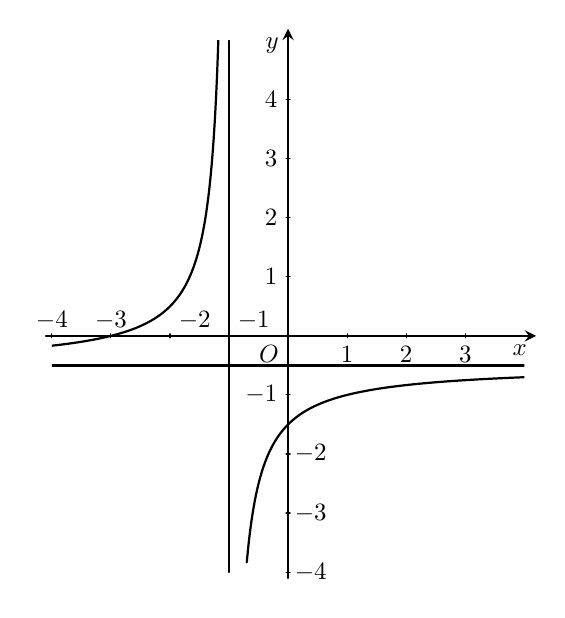
\begin{tikzpicture}[line join=round, line cap=round,>=stealth,thick,scale=0.75]
			\tikzset{every node/.style={scale=0.9}}
			\draw[->] (-4.1,0)--(4.2,0) node[below left] {$x$};
			\draw[->] (0,-4.1)--(0,5.2) node[below left] {$y$};
			\draw (0,0) node [below left] {$O$};
			\foreach \x/\nx in {1/1,2/2,3/3}
			\draw[thin] (\x,1pt)--(\x,-1pt) node [below] {$\nx$};
			\foreach \x/\nx in {-1/-1,-2/-2}
			\draw[thin] (\x,1pt)--(\x,-1pt) node [above right] {$\nx$};
			\foreach \x/\nx in {-4/-4,-3/-3}
			\draw[thin] (\x,1pt)--(\x,-1pt) node [above] {$\nx$};
			\foreach \y/\ny in {-1/-1,1/1,2/2,3/3,4/4}
			\draw[thin] (1pt,\y)--(-1pt,\y) node [left] {$\ny$};
			\foreach \y/\ny in {-4/-4,-3/-3,-2/-2}
			\draw[thin] (1pt,\y)--(-1pt,\y) node [right] {$\ny$};
			%\draw[dashed,thin](2,0)--(2,-6)--(0,-6);
			%\draw[dashed,thin] (1.01,-10)--(1.01,2);
			\begin{scope}
				\clip (-4,-4) rectangle (4,5);
				\draw[samples=200,domain=-5:-1.1,smooth,variable=\x] plot (\x,{(-1*(\x)-3)/(2*(\x)+2)});
				\draw[samples=200,domain=-.7:5,smooth,variable=\x] plot (\x,{(-1*(\x)-3)/(2*(\x)+2)});
				\draw (-1,-4)--(-1,5) (-5,-0.5)--(5,-0.5);
			\end{scope}
		\end{tikzpicture}}
	\loigiai{Dựa vào đồ thị, hàm số đồng biến trên từng khoảng xác định. Do đó $y'>0\, \forall x\ne -1$ suy ra $1-a>0\Rightarrow a<1$.
	}
\end{ex}

\begin{ex}%[BG12, Tran Tony]%[2D1H2-2]
	\immini{
		Cho hàm số bậc ba $y=f(x)$ có đồ thị như hình vẽ. Số điểm cực trị của hàm số $y=|f(x)|$ là
		\choice
		{$3$}
		{$2$}
		{$4$}
		{\True $5$}
	}
	{
		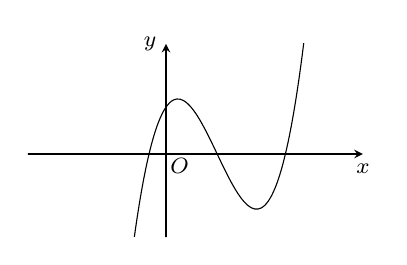
\begin{tikzpicture}[scale=0.5, font=\footnotesize, line join=round, line cap=round, >=stealth,yscale=0.7]
			\draw[->] (-3.5,0)--(5,0) node[below]{$x$} ;
			\draw[->] (0,-3)--(0,4) node[left]{$y$};
			\draw[fill=black] (0,0) circle(1pt) node[below right=-2pt] {$O$} ;
			\clip (-3.5,-3) rectangle (5,4) ;
			\draw[smooth, samples=100, domain=-3.5:5] plot(\x,{(\x-1.3)*(\x-1.3)*(\x-1.3) - 3*(\x-1.3)}) ;
		\end{tikzpicture}
	}
	\loigiai{
		\immini{
			Từ đồ thị hàm số $y=f(x)$, ta suy ra đồ thị hàm số $y=|f(x)|$ như hình vẽ bên. Dễ thấy hàm số $y=|f(x)|$ có $5$ điểm cực trị.
		}
		{
			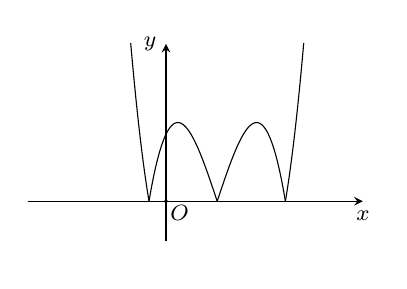
\begin{tikzpicture}[scale=0.5, font=\footnotesize, line join=round, line cap=round, >=stealth]
				\draw[->] (-3.5,0)--(5,0) node[below]{$x$} ;
				\draw[->] (0,-1)--(0,4) node[left]{$y$};
				\draw[fill=black] (0,0) circle(1pt) node[below right=-2pt] {$O$} ;
				\clip (-3.5,-1.5) rectangle (5,4) ;
				\draw[smooth, samples=100, domain=-3.5:-0.432051] plot(\x,{-(\x-1.3)*(\x-1.3)*(\x-1.3) + 3*(\x-1.3)}) ;
				\draw[smooth, samples=100, domain=-0.432051:1.3] plot(\x,{(\x-1.3)*(\x-1.3)*(\x-1.3) - 3*(\x-1.3)}) ;
				\draw[smooth, samples=100, domain=1.3:3.03205] plot(\x,{-(\x-1.3)*(\x-1.3)*(\x-1.3) + 3*(\x-1.3)}) ;
				\draw[smooth, samples=100, domain=3.03205:5] plot(\x,{(\x-1.3)*(\x-1.3)*(\x-1.3) - 3*(\x-1.3)}) ;
			\end{tikzpicture}
		}
	}
\end{ex}

\begin{ex}%[Dự án TL12New-4in1-NCT]%[2D1V4-2]
	Cho hàm số $y=\dfrac{2mx+m}{x-1}$. Tìm tất cả các giá trị của tham số $m$ để đường tiệm cận đứng, tiệm cận ngang của đồ thị hàm số cùng hai trục tọa độ tạo thành một hình chữ nhật có diện tích bằng $8$.
	\choice
	{$m\neq\pm 2$}
	{$m=\pm\dfrac{1}{2}$}
	{$m=2$}
	{\True $m=\pm 4$}
	\loigiai{
		Đồ thị hàm số có đường TCĐ là $x=1$ và đường TCN là $y=2m$.\\
		Diện tích hình chữ nhật tạo bởi hai đường tiện cận và hai trục tọa độ có diện tích bằng $8$ khi và chỉ khi \[1\cdot|2m|=8\Leftrightarrow m=\pm 4.\]}
\end{ex}

\begin{ex}%[2D1H5-7]
	Khoảng cách giữa hai điểm cực trị của đồ thị hàm số $y=\dfrac{x^2+x+1}{x+1}$ bằng
	\choice
	{\True $2\sqrt{5}$}
	{$2\sqrt{3}$}
	{$3\sqrt{2}$}
	{$5\sqrt{2}$}
	\loigiai{
		Tập xác định $\mathscr{D}=\mathbb{R}\setminus\{-1\}$.\\
		Ta có $y'=\dfrac{x^2+2x}{(x+1)^2}$ và $y'=0\Leftrightarrow x^2+2x=0\Leftrightarrow\hoac{& x=0 \\ & x=-2.}$
		\begin{center}
			
\begin{tikzpicture}
				\tkzTabInit[nocadre=false, lgt=1.2, espcl=2.5, deltacl=0.6]{$x$/0.6,$y'$/0.6,$y$/2}
				{$-\infty$, $-2$, $-1$, $0$, $+\infty$}
				\tkzTabLine {,+,0,-,d,-,0,+,}
				\tkzTabVar{-/$-\infty$, +/$-3$, -D+/$-\infty$ /$+\infty$,-/$1$, +/$+\infty$}
			\end{tikzpicture}
		\end{center}
		Từ bảng biến thiên ta có tọa độ hai điểm cực trị là $A(-2;-3)$ và $B(0;1)$.\\
		Vậy khoảng cách giữa hai điểm cực trị là $AB=2\sqrt{5}$.
	}
\end{ex}

\begin{ex}%[Mức độ N]%[2D1N4-1]
	Cho hàm số $y=f(x)$ có bảng biến thiên như sau
	\begin{center}
		
\begin{tikzpicture}
			\tkzTabInit[nocadre=false, lgt=1.5,espcl=4.5]
			{$x$/1,$f'(x)$/1,$f(x)$/2}
			{$-\infty$,$1$, $+\infty$}
			\tkzTabLine{,,d,,}
			\tkzTabVar{-/$3$, +D-/$+\infty$/$\--\infty$/,+/$3$/}
		\end{tikzpicture}
	\end{center}
	Tiệm cận đứng của đồ thị hàm số đã cho có phương trình là
	\choice
	{$x=-1$}
	{$x=-3$}
	{$x=3$}
	{\True $x=1$}
	\loigiai{Ta có $\lim\limits_{x \to 1^-}y=+\infty$; $\lim\limits_{x \to 1^+}y=-\infty$.\\
		Vậy tiệm cận đứng của đồ thị hàm số đã cho có phương trình là $x=1$.}
\end{ex}

\begin{ex}%[Mức độ 1]%[2D1N1-5]
	Đồ thị dưới mô tả sự thay đổi độ cao của một máy bay. Độ cao của máy bay giảm trong khoảng thời gian nào?
	\begin{center}
		\begin{tikzpicture}
			\pgfplotsset{/pgf/number format/use comma}
			\begin{axis}[
					title={Sự thay đổi độ cao của máy bay theo thời gian},
					title style={at={(1,1.2)},anchor=north east},
					xlabel={Thời gian (phút)},
					ylabel={Độ cao (mét)},
					xmin=0, xmax=100,
					ymin=0, ymax=12500,
					xtick={0,20,40,60,80,100},
					ytick={0,2500,5000,7500,10000,12500},
					%			yticklabel style={/pgf/number format/sci},
					legend pos=north west,
					ymajorgrids=true,
					grid style={dashed,black},
				]
				\addplot[
					color=black,
					domain=0:100,
					smooth
				]
				{500*x - 5*x^2};
			\end{axis}
		\end{tikzpicture}
	\end{center}
	\choice
	{$(0;50)$}
	{\True $(50;100)$}
	{$(0;100)$}
	{$(40;60)$}
	\loigiai{
		Từ đồ thị ta thấy độ cao máy bay giảm trong khoảng thời gian $(50;100)$ phút.
	}
\end{ex}

\begin{ex}%[2D1H5-3]
	\immini{Cho hàm số $y=f(x)$ có đồ thị như hình vẽ bên cạnh. Tìm $m$ để phương trình $f(x)=m$ có bốn nghiệm phân biệt.
		\choice
		{$-4<m\le -3$}
		{\True $-4<m<-3$}
		{$-4\le m<-3$}
		{$m>-4$}
	}{\begin{tikzpicture}[line cap=round,line join=round,>=stealth,x=1cm,
				y=1cm]
			% Vẽ 2 trục, điền các số lên trục
			\draw[->] (-3.08,0) -- (3.06,0); %Vẽ trục Ox
			\foreach \x in {1,-1} %Đánh số trên trục
			\draw[shift={(\x,0)},color=black] (0pt,2pt) -- (0pt,-2pt)
			node[above] { $\x$};
			\draw[->,color=black] (0,-5.06) -- (0,0.98); %Vẽ trục Oy
			\foreach \y in {-3,-4} %đánh số trên trục
			\draw[shift={(0,\y)},color=black] (2pt,0pt) -- (-2pt,0pt)
			node[above left] {\normalsize $\y$};
			\draw[color=black] (3,.2) node[right] {\normalsize $x$}; %đặt tên trục
			\draw[color=black] (.1,0.8) node[right] {\normalsize $y$}; %đặt tên trục
			\draw[color=black] (0pt,-8pt) node[right] {\normalsize $O$}; %gốc tọa độ
			\clip(-3.08,-4.06) rectangle (2.06,0.98); %cắt khung đồ thị
			%Vẽ đồ thị
			\draw[smooth,samples=100,domain=-2.08:2.06]
			plot(\x,{(\x)^4-2*(\x)^2-3}); %Vẽ đồ thị
			% Vẽ thêm mấy cái râu ria
			\draw[dashed] (-1,0)--(-1,-4)--(1,-4)--(1,0);
			%Vẽ dấu chấm tròn
			\fill (0cm,0cm) circle (1.5pt);
		\end{tikzpicture}}
	\loigiai{
		Từ đồ thị ta thấy  phương trình $f(x)=m$ có bốn ngiệm phân biệt khi $-4<m<-3$.}
\end{ex}

\begin{ex}%[2D1H2-7]
	Giả sử chi phí tiền xăng C (đồng) phụ thuộc tốc độ trung bình  $v\left( {{\rm{\;km}}/{\rm{h}}} \right)$ theo công thức
	\[C(v) = \dfrac{16000}{v} + \dfrac{5}{2}v \quad (0 < v \le 120)\]
	Tính tốc độ trung bình để chi phí tiền xăng đạt cực tiểu.
	\choice
	{$60$ km/h}
	{$70$ km/h}
	{$50$ km/h}
	{\True $80$ km/h}
	\loigiai{
		Tập xác định: $D=(0; 120]$.\\
		Đạo hàm $C'(v)=-\dfrac{16000}{v^2}+\dfrac{5}{2}=\dfrac{5(v-80)(v+80)}{2v^2}$; $C'(v)=0\Leftrightarrow v=-80$ (loại) hoặc $v=80$.\\
		Bảng biến thiên
		\begin{center}
			
\begin{tikzpicture}[>=stealth]
				\tkzTabInit[nocadre=false,lgt=1.5,espcl=2,deltacl=0.5]{$v$/.7 ,$C'(v)$/.7,$C(v)$/2}
				{$0$ , $80$ , $120$}
				\tkzTabLine{ d, - , $0$ , + , }
				\tkzTabVar{+D+/$ $/$+\infty$ , -/$400$ , +/$\dfrac{1300}{3}$}
			\end{tikzpicture}
		\end{center}
		Quan sát bảng biến thiên, ta nhận thấy hàm số đạt cực tiểu khi $v=80$.\\
		Như vậy, để chi phí tiền xăng đạt cực tiểu, tài xế nên chạy xe với tốc độ trung bình là $80$ km/h.
	}
\end{ex}

\begin{ex}%[Mức độ 3]%[BG12-4IN1, Nguyễn Khánh Trọng]%[2D1V3-6]
	Ông An dự định làm một cái bể chứa nước hình trụ bằng inox có nắp đậy với thể tích là $k$ m$^3$ $(k>0)$. Chi phí mỗi m$^2$ đáy là $600$ nghìn đồng, mỗi m$^2$ nắp là $200$ nghìn đồng và mỗi m$^2$ mặt bên là $400$ nghìn đồng. Hỏi ông An cần chọn bán kính đáy của bể là bao nhiêu để chi phí làm bể là ít nhất? (Biết bề dày vỏ inox không đáng kể)
	\choice
	{$\sqrt[3]{\dfrac{k}{\pi}}$}
	{$\sqrt[3]{\dfrac{2\pi}{k}}$}
	{\True $\sqrt[3]{\dfrac{k}{2\pi}}$}
	{$\sqrt[3]{\dfrac{k}{2}}$}
	\loigiai{
		\immini{
			Gọi $r, h$ $(r,h>0)$ lần lượt là bán kính đáy và chiều cao của hình trụ.\\
			Thể tích khối trụ $V=\pi r^2h=k\Rightarrow h=\dfrac{k}{\pi r^2}$.\\
			Diện tích đáy và nắp là $S_d=S_n=\pi r^2$; diện tích xung quanh là $S_{xq}=2\pi rh$.\\
			Khi đó chi phí làm bể là\\
			\[C=(600+200)\pi r^2+400\cdot 2\pi rh=800\pi r^2+800\pi r\dfrac{k}{\pi r^2}=800\left(\pi r^2+\dfrac{k}{r}\right).\]
		}{
			\begin{tikzpicture}[scale=0.7, font=\footnotesize, line join=round, line cap=round, >=stealth]
				\def \x{1.8} %bán kính trục lớn elip
				\def \y{0.8} %bán kính trục bé elip
				\def \h{3.5} %chiều cao hình trụ
				\coordinate (A) at (0,0);
				\coordinate (B) at (2*\x,0);
				\coordinate (O) at ($(A)!0.5!(B)$);
				\coordinate (O') at ($(O)+(0,\h)$);
				\coordinate (A') at ($(A)+(0,\h)$);
				\coordinate (B') at ($(B)+(0,\h)$);
				\draw[dashed] (B) arc(0:180:\x cm and \y cm);
				\draw (B) arc(0:-180:\x cm and \y cm);
				\draw (O') ellipse (\x cm and \y cm);
				\coordinate (I) at ($(O)+(-30:\x cm and \y cm)$);
				\tkzDrawSegments(A,A' B,B')
				\tkzDrawSegments[dashed](O,I)
				\tkzDrawPoints[fill=black,size=3](O)
				\tkzLabelSegment[above](O,I){$r$}
				\draw[<->] (-0.7,0)--(-0.7,\h);
				\node at (-0.7,\h/2) [left]{$h$};
			\end{tikzpicture}
		}
		\noindent
		Đặt $f(r)=\pi r^2+\dfrac{k}{r}$, $r>0\Rightarrow f'(r)=2\pi r-\dfrac{k}{r^2}=\dfrac{2\pi r^3-k}{r^2}$;\\
		Ta có $f'(r)=0\Leftrightarrow r=\sqrt[3]{\dfrac{k}{2\pi}}$, $(k>0)$.\\
		Lập bảng biến thiên, ta thấy $f(r)$ đạt giá trị nhỏ nhất khi $r=\sqrt[3]{\dfrac{k}{2\pi}}$.\\
		Vậy với bán kính đáy là $r=\sqrt[3]{\dfrac{k}{2\pi}}$ thì chi phí làm bể là ít nhất.}
\end{ex}

\begin{ex}%[Dự Án Giảng 12 4 in 1, Lê Văn Toàn]%[2D1CV5-6]%[2D1V5-6]
	Cho hàm số $y=\dfrac{x+2}{x+1}$ có đồ thị $(C)$. Gọi $d$ là khoảng cách từ giao điểm hai tiệm cận của đồ thị $(C)$ đến một tiếp tuyến của $(C)$. Giá trị lớn nhất của $d$ có thể đạt được là
	\choice
	{$\sqrt{3}$}
	{\True $\sqrt{2}$}
	{$3\sqrt{3}$}
	{$2\sqrt{2}$}
	\loigiai{
		Ta có $y=\dfrac{x+2}{x+1}\Rightarrow y'=\dfrac{-1}{(x+1)^2}$.\\
		Đồ thị $(C)$ của hàm số $y=\dfrac{x+2}{x+1}$ có đường tiệm cận đứng là $x=-1$ và đường tiệm cận ngang là $y=1$.\\
		Suy ra giao điểm hai đường tiệm cận là $I(-1;1)$.\\
		Lấy $M(x_0;y_0)\in (C)$ tùy ý với $x_0\ne -1$, $y_0=\dfrac{x_0+2}{x_0+1}$.\\
		Ta có tiếp tuyến của đồ thị $(C)$ tại điểm $M(x_0;y_0)$ là
		\[\Delta\colon y=\dfrac{-1}{(x_0+1)^2}(x-x_0)+y_0\Leftrightarrow \Delta\colon x+(x_0+1)^2y-x_0^2-4x_0-2=0.\]
		Khoảng cách từ điểm $I$ đến tiếp tuyến của đồ thị $(C)$ tại điểm $M(x_0;y_0)$ là
		\allowdisplaybreaks
		\begin{eqnarray*}
			d=\mathrm{d}(I,\Delta)&=&\dfrac{\left|-1+(x_0+1)^2-x_0^2-4x_0-2\right|}{\sqrt{1+(x_0+1)^4}}\\
			&=&\dfrac{2|x_0+1|}{\sqrt{1+(x_0+1)^4}}\\
			&=&\dfrac{2}{\sqrt{\dfrac{1}{(x_0+1)^2}+(x_0+1)^2}}\\
			&\le& \dfrac{2}{\sqrt{2\sqrt{\dfrac{1}{(x_0+1)^2}\cdot (x_0+1)^2}}}=\sqrt{2}.
		\end{eqnarray*}
		Dấu ``$=$'' xảy ra khi và chỉ khi $\dfrac{1}{(x_0+1)^2=(x_0+1)^2}\Leftrightarrow (x_0+1)^4=1\Leftrightarrow \hoac{&x_0=0\\&x_0=-2}$ (nhận).\\
		Vậy giá trị lớn nhất của $d$ có thể đạt được là $\sqrt{2}$.
	}
\end{ex}

\begin{ex}%[TEX NBV, Trương Đăng Khoa]%[2D1V3-6]
	\immini{Cho nửa đường tròn đường kính $AB=2$ và hai điểm $C$, $D$ thay đổi trên nửa đường tròn đó sao cho $ABCD$ là hình thang. Diện tích lớn nhất của hình thang $ABCD$ bằng
		\choice
		{ $\dfrac{1}{2}$}
		{ \True $\dfrac{3\sqrt{3}}{4}$}
		{ $1$}
		{ $\dfrac{3\sqrt{3}}{2}$
		}}{
		\begin{tikzpicture}[scale=1, font=\footnotesize, line join=round, line cap=round,>=stealth]
			\coordinate (O) at (2.5,0);
			\coordinate (A) at (0,0);
			\coordinate (B) at (5,0);
			\coordinate (D) at ($(O) + (120:2.5)$);
			\coordinate (C) at ($(O) + (60:2.5)$);
			\coordinate (I) at ($(D)!0.5!(C)$);
			\coordinate (H) at ($(A)!(D)!(O)$);
			\draw (5,0) arc (0:180:2.5);
			\draw (A)--(B)--(C)--(D)--(A) (O)--(I) (O)--node[above]{$1$}(D) (D)--node[left]{$x$}(H);
			\draw pic[draw,angle radius=0.3cm]{right angle=D--H--A};
			\draw pic[draw,angle radius=0.3cm]{right angle=I--O--B};
			\foreach \x/\y in {A/-90, B/-90, D/90,C/90, I/-45,O/-90, H/-90}{\fill (\x) circle(1.2pt) ($(\x)+(\y:0.3cm)$) node{$\x$};}
		\end{tikzpicture}
	}
	\loigiai{
		Gọi $H$ là hình chiếu vuông góc của $D$ lên $AB$, $I$ là trung điểm của đoạn $CD$ và $O$ là trung điểm của $AB$.\\
		Đặt $DH=x$, $0<x<1$.\\
		Ta có $DC=2DI=2OH=2\sqrt{OD^2-DH^2}=2\sqrt{1-x^2}$.\\
		Diện tích của hình thang $ABCD$ là $S=f( x )=\dfrac{( AB+CD )\cdot DH}{2}=\left( 1+\sqrt{1-x^2}\right)x$.\\
		Ta có $f'( x )=\dfrac{\sqrt{1-x^2}+1-2x^2}{\sqrt{1-x^2}}$.\\
		$f'( x )=0\Leftrightarrow \sqrt{1-x^2}+1-2x^2=0$. ($\ast$)\\
		Đặt $t=\sqrt{1-x^2}$, ($t\ge 0$) khi đó phương trình ($\ast$) trở thành $2t^2+t-1=0\Leftrightarrow \hoac{
				& t=-1 \text{ (loại)}\\
				& t=\dfrac{1}{2}.
			}$\\
		Khi đó  $\sqrt{1-x^2}=\dfrac{1}{2}\Leftrightarrow x^2=\dfrac{3}{4}\Leftrightarrow x=\pm \dfrac{\sqrt{3}}{2}$.\\
		Bảng biến thiên
		\begin{center}
			
\begin{tikzpicture}[scale=1, font=\footnotesize]
				\tkzTabInit[nocadre=false, lgt=1.2, espcl=2, deltacl=0.6]
				{$x$/0.8,$f'(x)$/0.6,$f(x)$/2}
				{$0$,$\dfrac{\sqrt{3}}{2}$,$1$};
				\tkzTabLine{,+,$0$,-,};
				\tkzTabVar{-/$0$,+/$\dfrac{3\sqrt{3}}{4}$,-/$1$};
			\end{tikzpicture}
		\end{center}
		Vậy diện tích lớn nhất của hình thang $ABCD$ bằng $\dfrac{3\sqrt{3}}{4}$.}
\end{ex}

\begin{ex}%[BG-12NEW-4in1, Nguyen Huynh]%[2D1H4-1]
	Trong mặt phẳng $Oxy$, tổng khoảng cách từ gốc tọa độ đến tất cả các đường tiệm cận của đồ thị hàm số $y=\log_2\dfrac{2x+3}{x-1}$ bằng
	\choice
	{$2$}
	{$3$}
	{$\dfrac{5}{2}$}
	{\True $\dfrac{7}{2}$}
	\loigiai{
		Điều kiện $\dfrac{2x+3}{x-1}>0\Leftrightarrow\hoac{&x>1\\&x<-\dfrac{3}{2}.}$\\
		Ta xét các giới hạn sau
		\begin{itemize}
			\item $\lim\limits_{x\to{1^+}}\left(\log_2\dfrac{2x+3}{x-1}\right)=+\infty$.
			\item $\lim\limits_{x\to{\left(-\tfrac{3}{2}\right)^-}}\left(\log_2\dfrac{2x+3}{x-1}\right)=-\infty$.
		\end{itemize}
		Từ đó suy ra tiệm cận đứng là $d_1\colon x=-\dfrac{3}{2}$; $d_2\colon x=1$.\\
		Mặt khác $\lim\limits_{x\to+\infty}\left(\log_2\dfrac{2x+3}{x-1}\right)=\lim\limits_{x\to-\infty}\left(\log_2\dfrac{2x+3}{x-1}\right)=1$.\\
		Từ đó suy ra tiệm cận ngang là $\left(d_3\right)\colon y=1$.\\
		Ta có $T=\mathrm{d}\left(O,d_1\right)+\mathrm{d}\left(O,d_2\right)+\mathrm{d}\left(O,d_3\right)=\dfrac{3}{2}+1+1=\dfrac{7}{2}$.}
\end{ex}

\begin{ex}%[Dự án Giảng 12 Nhóm Toán & LaTex, Lê Minh Thiện Anh]%[2D1N5-1]
	\immini{Đường cong bên là đồ thị của một trong bốn hàm số đã cho sau đây. Hỏi đó là hàm số nào?
		\choice
		{$y=-x^3+x^2-2$}
		{\True $y=x^3+3x^2-2$}
		{$y=x^3-3x+2$}
		{$y=x^2-3x-2$}
	}{
		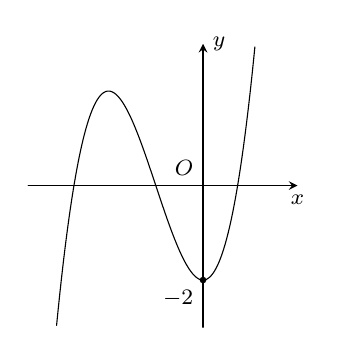
\begin{tikzpicture}[scale=0.6, font=\footnotesize,line join=round, line cap=round,>=stealth]
			\draw[->] (-3.7,0.) -- (2,0) node[below]{$x$};
			\draw[->] (0,-3) -- (0,3) node[right]{$y$};
			\fill (0,0) node[above left]{$O$};
			\fill (0,-2) circle(2pt) node[below left]{$-2$};
			\draw[smooth,samples=300,domain=-3.1:1.1] plot(\x,{(\x+2)^3-3*(\x+2)^2+2});
		\end{tikzpicture}
	}
	\loigiai{
		Dựa vào hình dáng đồ thị, ta thấy đây là đồ thị của hàm số bậc ba $y=ax^3+bx^2+cx+d$ với $a>0$ nên loại các hàm $y=x^2-3x-2$, $y=-x^3+x^2-2$.\\
		Mặt khác, đồ thị đi qua điểm $(0;-2)$ nên loại hàm $y=x^3-3x+2$.
	}
\end{ex}

\begin{ex}%[2D1N5-1]
	Bảng biến thiên sau là của hàm số nào dưới đây?
	\begin{center}
		
\begin{tikzpicture}
			\tkzTabInit[nocadre=true,espcl=2.5,lgt=1.2,deltacl=0.5]
			{$x$/0.7,$y'$/0.7,$y$/2}
			{$-\infty$,$0$,$1$,$2$,$+\infty$}
			\tkzTabLine{,+,$0$,-,d,-,$0$,+,}
			\tkzTabVar{-/$-\infty$,+/$2$,-D+/$-\infty$/$+\infty$,-/$6$,+/$+\infty$}
		\end{tikzpicture}
	\end{center}
	\choice
	{$y=\dfrac{x^2-4x+2}{x-1}$}
	{\True $y=\dfrac{x^2+2x-2}{x-1}$}
	{$y=\dfrac{x^2+2x-2}{x+1}$}
	{$y=\dfrac{x^2+2}{x-1}$}
	\loigiai{
		Từ bảng biến thiên ta thấy $\heva{&\lim\limits_{x\to 1^-}y=-\infty\\&\lim\limits_{x\to 1^+}y=+\infty}\Rightarrow x=1$ là đường tiệm cận đứng nên loại đáp án \textbf{C}.\\
		Đồ thị hàm số có điểm cực đại $(0;2)$ nên loại đáp án \textbf{D}.\\
		Đồ thị hàm số có điểm cực tiểu $(2;6)$ nên loại đáp án \textbf{A}.
	}
\end{ex}

\begin{ex}%[BG-12NEW-4in1, Nguyen Huynh]%[2D1N4-1]
	Tiệm cận xiên của đồ thị hàm số $y=\dfrac{x^2+3x+5}{x+2}$ là
	\choice
	{$y=x$}
	{$y=x+1$}
	{\True $y=x+2$}
	{$y=x+3$}
	\loigiai{
		Tập xác định của hàm số là $\mathbb{R}\setminus\{-2\}$.
		Ta thấy
		\begin{itemize}
			\item $\lim\limits_{x\to +\infty}\dfrac{x^2+3x+5}{x(x+2)}=\lim\limits_{x\to +\infty}\dfrac{1+\tfrac{3}{x}+\tfrac{5}{x^2}}{1+\tfrac{2}{x}}=1$.\\
			\item $\lim\limits_{x\to+\infty}(y-x)=\lim\limits_{x\to +\infty}\dfrac{2x+3}{x+2}=2$.
		\end{itemize}
		Vậy $y=x+2$ là tiệm cận xiên của đồ thị hàm số.\\
		Tương tự, ta thấy $y=x+2$ là tiệm cận xiên của đồ thị hàm số.\\
		Vậy $y=x+2$ là tiệm cận xiên của đồ thị hàm số.

	}
\end{ex}

\begin{ex}%[BG-12NEW-4in1, Nguyen Huynh]%[2D1H4-1]
	Cho hàm số $y=a^x$ với $0<a\ne1$. Mệnh đề nào sau đây \textbf{sai}?
	\choice
	{Đồ thị hàm số $y=a^x$ và đồ thị hàm số $y=\log_ax$ đối xứng nhau qua đường thẳng $y=x$}
	{Hàm số $y=a^x$ có tập xác định là $\mathbb{R}$ và tập giá trị là $(0;+\infty)$}
	{Hàm số $y=a^x$ đồng biến trên tập xác định của nó khi $a>1$}
	{\True Đồ thị hàm số $y=a^x$ có tiệm cận đứng là trục tung}
	\loigiai{Theo lý thuyết, ta có $\lim\limits_{x\to0^+}a^x=1$ và $\lim\limits_{x\to0^-}a^x=1$ nên không nhận trục tung làm tiệm cận đứng.}
\end{ex}

\begin{ex}%[Khảo sát chất lượng L1 - THPT Nguyễn Viết Xuân - Vĩnh Phúc - 2019, Mức độ H]%[Dự án giảng 12 - Trung Anh]%[2D1H2-5]
	Biết đồ thị hàm số $y = x^4 - 2mx^2 + 2$ có ba điểm cực trị là ba đỉnh của một tam giác vuông cân. Tính giá trị của biểu thức $P = m^2 + 2m + 1$.
	\choice
	{$P = 1$}
	{\True $P = 4$}
	{$P = 2$}
	{$P = 0$}
	\loigiai{
		Tập xác định: $\mathscr{D} = \mathbb{R}$.
		$y' = 4x^3 - 4mx$.\\
		$y' = 0 \Leftrightarrow \hoac{&x = 0 \\	&x^2 = m.}$\\
		Hàm số có ba điểm cực trị $\Leftrightarrow m > 0$.\\
		Khi đó ba điểm cực trị của hàm số là $x_1 = 0$, $x_2 = \sqrt{m}$, $x_3 = -\sqrt{m}$.\\
		Vậy ba điểm cực trị của đồ thị hàm số là $A(0;2)$, $B\left(\sqrt{m}; 2 - m^2 \right)$, $C\left(-\sqrt{m}; 2 - m^2 \right)$. Ba điểm này luôn tạo thành tam giác cân tại $A$. Vậy tam giác này vuông cân khi và chỉ khi $\widehat{BAC} = 90^\circ$.\\
		Tương đương $\overrightarrow{AB} \cdot \overrightarrow{AC} = 0$, hay $\sqrt{m} \cdot \left(-\sqrt{m}\right) + (-m^2) \cdot (-m^2) = 0$.\\
		Giải phương trình này ta có $m = 1$ là nghiệm duy nhất. Do đó $P = 4$.
	}
\end{ex}
\begin{ex}%[SGK12-KNTT ]%[2D1H5-8]
	Khi máu di chuyển từ tim qua các động mạch chính rồi đến các mao mạch và quay trở lại qua các tĩnh mạch, huyết áp tâm thu (tức là áp lực của máu lên động mạch khi tim co bóp) liên tục giảm xuống. Giả sử một người có huyết áp tâm thu $P$ (tính bằng mmHg) được cho bởi hàm số
	\[
		P(t)=\dfrac{25 t^2+125}{t^2+1}, 0 \leq t \leq 10,
	\]
	trong đó thời gian $t$ được tính bằng giây. Tính tốc độ thay đổi của huyết áp sau $5$ giây kể từ khi máu rời tim.
	\choice
	{$-\dfrac{20}{17}$}
	{\True $-\dfrac{250}{169}$}
	{$-\dfrac{120}{163}$}
	{$-\dfrac{19}{132}$}
	\loigiai{
		Ta có tốc độ thay đổi của huyết áp là $P'(t)=\dfrac{-200t}{(t^2+1)^2}$.\\
		Do đó tốc độ thay đổi huyết áp sau $5$ giây là $P'(5)=-\dfrac{250}{169}$.
	}
\end{ex}
\begin{ex}%[KNTT]giảng 12 New-4in1, Toàn Phan]%[2D1H5-8]KNTT
	Khi bỏ qua sức cản của không khí, độ cao (mét) của một vật được phóng thẳng đứng lên trên từ điểm cách mặt đất $2$ m với vận tốc ban đầu $24{,}5$ m/s là $h(t)=2+24{,}5t-4{,}9t^2$ (theo Vật lí đại cương, NXB Giáo dục Việt Nam, $2016$). Tìm vận tốc của vật sau $2$ giây.
	\choice
	{\True $4{,}9$}
	{$3{,}2$}
	{$1{,}3$}
	{$5{,}5$}
	\loigiai{
	Theo ý nghĩa cơ học của đạo hàm, vận tốc của vật là $v=h'(t)=24{,}5-9{,}8t$ m/s.\\
	Do đó, vận tốc của vật sau $2$ giây là $v(2)=24{,}5-9{,}8\cdot 2=4{,}9$ m/s.
	}
\end{ex}

\TL

\begin{ex}%[SGK12-CTST, Mức độ 2]%[2D1H2-1]
	Tìm cực trị của hàm số $g(x)=\dfrac{x^2+x+4}{x+1}$.
	\loigiai{
		Tập xác định $\mathscr{D}=\mathbb{R}\setminus \{-1\}$.\\
		Ta có $g(x)=x+\dfrac{4}{x+1} \Rightarrow g'(x)=1-\dfrac{4}{(x+1)^2}=\dfrac{x^2+2x-3}{(x+1)^2}$;\\
		$g'(x)=0 \Leftrightarrow x^2+2x-3=0 \Leftrightarrow \hoac{& x=-3\\& x=1.}$\\
		Bảng biến thiên
		\begin{center}
			
\begin{tikzpicture}
				\tkzTabInit[nocadre=false,lgt=1.2,espcl=2.5,deltacl=0.6]
				{$x$ /0.6,$g'(x)$ /0.6,$g(x)$ /2}
				{$-\infty$,$-3$,$-1$,$1$,$+\infty$}
				\tkzTabLine{,+,$0$,-,d,-,$0$,+,}
				\tkzTabVar{-/$-\infty$,+/$-5$,-D+/$-\infty$/$+\infty$,-/$3$,+/$+\infty$}
			\end{tikzpicture}
		\end{center}
		Vậy hàm số đạt cực đại tại $x=-3$, $y_{\text{CĐ}}=g(-3)=-5$; và hàm số đạt cực tiểu tại $x=1$, $y_{\text{CT}}=g(1)=3$.
	}
\end{ex}
\begin{ex}%[SGK12-CTST, Mức độ 2]%[2D1H1-5]
	Kim ngạch xuất khẩu rau quả của Việt Nam trong các năm từ $2010$ đến $2017$ có thể được tính xấp xỉ bằng công thức $f(x)=0{,}01x^3-0{,}04x^2+0{,}25x+0{,}44$ (tỉ USD) với $x$ là số năm tính từ $2010$ đến $2017$ $(0\leq x\leq 7)$.
	\begin{flushright}
		(\textit{Theo:} https://infographics.vn/interactive-xuat-khau-rau-qua-
		du-bao-bung-no-dat-4-ty-usd-trong-nam-2023/116220.vna)
	\end{flushright}
	\begin{enumerate}
		\item Tính đạo hàm của hàm số $y=f(x)$.
		\item Chứng minh rằng kim ngạch xuất khẩu rau quả của Việt Nam tăng liên tục trong các năm từ $2010$ đến $2017$.
	\end{enumerate}
	\loigiai{
		\begin{enumerate}
			\item Ta có $f'(x)=0{,}03x^2-0{,}08x+0{,}25$.
			\item Xét $f'(x)=0 \Leftrightarrow 0{,}03x^2-0{,}08x+0{,}25=0$ (vô nghiệm).\\
			      Bảng biến thiên
			      \begin{center}
				      
\begin{tikzpicture}
					      \tkzTabInit[nocadre=false,lgt=1.2,espcl=5,deltacl=0.6]
					      {$x$ /0.6,$f'(x)$ /0.6,$f(x)$ /2}
					      {$0$,$7$}
					      \tkzTabLine{,+,}
					      \tkzTabVar{-/$0{,}44$,+/$3{,}66$}
				      \end{tikzpicture}
			      \end{center}
			      Từ bảng biến thiên trên, ta thấy $f'(x)>0$, $\forall x\in [0;7]$.\\
			      Vậy kim ngạch xuất khẩu rau quả của Việt Nam tăng liên tục trong các năm từ $2010$ đến $2017$.
		\end{enumerate}
	}
\end{ex}
\begin{ex}%[Mức độ 4]%[BG12-4IN1, Nguyễn Khánh Trọng]%[2D1C3-6]
	\immini[thm]{
		Cho một tấm gỗ hình vuông cạnh $200$ cm. Người ta cắt một tấm gỗ có hình một tam giác vuông $ABC$ từ tấm gỗ hình vuông đã cho như hình vẽ bên. Biết $AB=x$ ($0<x<60$ cm) là một cạnh góc vuông của tam giác $ABC$ và tổng độ dài cạnh góc vuông $AB$ với cạnh huyền $BC$ bằng $120$ cm. Tìm $x$ để tam giác $ABC$ có diện tích lớn nhất.
		% \shortans{$40$}
	}{
		\begin{tikzpicture}[scale=0.72, font=\footnotesize, line join=round, line cap=round, >=stealth]
			\draw[dashed] (0,0)--(4,0)--(0,1)--(0,0);
			\draw (4,0)--(5,0)--(5,5)--(0,5)--(0,1);
			\node at (0,0.5)[below left] {$x$}; \node at (2,0.5)[above,rotate=-13] {$120-x$}; \node at (2.5,5)[above] {$200$};
			\fill (0,0) circle (1.5pt) node[below left]{$A$} (4,0) circle (1.5pt) node[below]{$C$} (0,1) circle (1.5pt) node[left]{$B$};
		\end{tikzpicture}
	}

	\loigiai{
		Độ dài cạnh huyền $BC$ là $120-x$.\\
		Khi đó độ dài cạnh $AC=\sqrt{BC^2-AB^2}=\sqrt{(120-x)^2-x^2}=\sqrt{14400-240x}$.\\
		Diện tích tam giác $ABC$ là $S=\dfrac{1}{2}AB\cdot AC=\dfrac{1}{2}x\sqrt{14400-240x}$.\\
		Xét hàm số $f(x)=x\sqrt{14400-240x}$ với $0<x<60$.\\
		Ta có $f'(x)=\sqrt{14400-240x}-\dfrac{120x}{\sqrt{14400-240x}}=\dfrac{14400-360x}{\sqrt{14400-240x}}$;\\
		$f'(x)=0\Leftrightarrow x=40\in(0;60)$.\\
		Bảng biến thiên
		\begin{center}
			
\begin{tikzpicture}
				\tkzTabInit[nocadre=false,lgt=1.2,espcl=2.5,deltacl=0.6]
				{$x$ /0.6,$f'(x)$ /0.6,$f(x)$ /2}
				{$0$,$40$,$60$}
				\tkzTabLine{,+,$0$,-,}
				\tkzTabVar{-/, +/,-/}
			\end{tikzpicture}
		\end{center}
		Vậy tam giác $ABC$ có diện tích lớn nhất khi $AB=40$ cm.
	}
\end{ex}
\begin{ex}%[Dự án đề ôn tập GK1, Mui Doan]%[2D1V3-6]
	Có hai xã $A$, $B$ cùng ở một bên bờ sông Lam, khoảng cách từ hai xã đó đến bờ sông lần lượt là $AA'=500$  m, $BB'=600$  m và người ta đo được $A'B'=2\,200$  m. Các kĩ sư muốn xây một trạm cung cấp nước sạch nằm bên bờ sông Lam cho dân hai xã. Để tiết kiệm chi phí, các kĩ sư cần phải chọn vị trí $M$ của trạm cung cấp nước sạch đó trên đoạn $A'B'$ sao cho tổng khoảng cách từ hai xã đến vị trí $M$ là nhỏ nhất. Hãy tìm vị trí tối ưu đó.
	% \shortans{$2460$}
	\begin{center}
		\begin{tikzpicture}
			\path
			(0:0) coordinate (A')
			(0:6) coordinate (B')
			(0:2) coordinate (M)
			($(A')+(90:2.5)$) coordinate (A)
			($(B')+(90:3)$) coordinate (B)
			;
			\fill[cyan!50] (-1.5,-1) rectangle (7.5,0);
			\draw[thick] (A')--node[left]{$500$ m}(A)--(M)--(B)--node[right]{$600$ m}(B');

			\foreach \i/\j in{A'/-100,B'/-80,A/100,B/80,M/-90}{\fill [black](\i) circle (1pt) ($(\i)+(\j:3mm)$) node {$\i$};}

			\draw [dashed,<->]	(0,.6)--(6,.6) node[pos=0.75,sloped,above]{$2\,200$ m};
		\end{tikzpicture}
	\end{center}
	\loigiai{
		\begin{center}
			\begin{tikzpicture}
				\path
				(0:0) coordinate (A')
				(0:6) coordinate (B')
				(0:2) coordinate (M)
				($(A')+(90:2.5)$) coordinate (A)
				($(B')+(90:3)$) coordinate (B)
				;
				\draw[thick] (A')--node[left]{$500 \text{(m)}$}(A)--(M)--(B)--node[right]{$600 \text{(m)}$}(B') (A')--(B');

				\foreach \i/\j in{A'/-100,B'/-80,A/100,B/80,M/-90}{\fill [black](\i) circle (1pt) ($(\i)+(\j:3mm)$) node {$\i$};}

				\draw [dashed,<->]	(0,.6)--(6,.6) node[pos=0.75,sloped,above]{$2\,200\text{(m)}$}; %Tùy chọn sloped,above,below
				\node at (3,-1.5){\it Hình 37};
			\end{tikzpicture}
		\end{center}
		Đặt $A'M=x$, $(0<x<2200)$,  $B'M=2200-x$.\\
		Ta có  $AM=\sqrt{x^2+500^2}$, $BM=\sqrt{(2200-x)^2+600^2}$.\\
		Khi đó tổng khoảng cách từ hai xã đến vị trí $M$ là $AM+BM= \sqrt{x^2+500^2}+\sqrt{(2200-x)^2+600^2} $.\\
		Xét hàm số $f(x)= \sqrt{x^2+500^2}+\sqrt{(2200-x)^2+600^2}$ trên khoảng $(0<x<2200)$.\\
		%$f(x)=\sqrt{x^2+500}+\sqrt{x^2-4400x+4840600}$ .\\
		$f'(x)=\dfrac{x}{\sqrt{x^2+500^2}}-\dfrac{2200-x}{\sqrt{(2200-x)^2+600^2}}$,
		\allowdisplaybreaks
		\begin{eqnarray*}
			f'(x)=0&\Leftrightarrow&\dfrac{x}{\sqrt{x^2+500^2}}=\dfrac{2200-x}{\sqrt{(2200-x)^2+600^2}}
			\\
			&\Leftrightarrow&\dfrac{x^2}{x^2+500^2}=\dfrac{(2200-x)^2}{(2200-x)^2+600^2}\\
			&\Leftrightarrow&\dfrac{x^2+500^2}{x^2}=\dfrac{(2200-x)^2+600^2}{(2200-x)^2}\\
			&\Leftrightarrow& 1+\dfrac{500^2}{x^2}=1+\dfrac{600^2}{(2200-x)^2}
			\\
			&\Leftrightarrow& \dfrac{25}{x^2}=\dfrac{36}{(2200-x)^2}
			\\
			&\Leftrightarrow& \dfrac{5}{x}=\dfrac{6}{2200-x}
			\\
			&\Leftrightarrow& x=1\,000~ \text{vì}~  x>0.
		\end{eqnarray*}
		Bảng biến thiên hàm số $f(x)$ trên khoảng $( 0;2\,200)$.
		\begin{center}
			
\begin{tikzpicture}
				\tkzTabInit[lgt=1.2,espcl=4.5,deltacl=0.6]
				{$x$/1,$f'(x)$/1,$f(x)$/3} {$0$,$1000$,$2200$}
				\tkzTabLine{,-,0,+,}
				\tkzTabVar{+/$2780$,-/$2460$,+/$2856$}
			\end{tikzpicture}
		\end{center}
		Vậy giá trị nhỏ nhất của tổng khoảng cách từ hai xã đó đến bờ sông  là khoảng $2\,460$  m, tại vị trí $M$ cách điểm $A'$  là $1\,000$  m.
	}
\end{ex}
\Closesolutionfile{ans}

% \begin{indapan}
% 	{ans/ansc1l4}
% \end{indapan}

